%%%%%%%%%%%%%%%%%%%%%%%%%%%%%%%%%%%%%%%%%%%%%%%%%%%%%%%%%%%%%%%%%%%%%%%%%%%%%%%%%%
\begin{frame}[fragile]\frametitle{}
\begin{center}
{\Large Deep Q Learning}
\end{center}
\end{frame}

%%%%%%%%%%%%%%%%%%%%%%%%%%%%%%%%%%%%%%%%%%%%%%%%%%%%%%%%%%%%%%%%%%%%%%%%%%%%%%%%%%
\begin{frame}[fragile]\frametitle{Problems with Q Learning}


\begin{itemize}
\item Q Learning is suitable for small states space, tabular methods
\item Inefficient for Large and continuous state space problems.
\item Not enough time, resources.
\item Deep Learning comes to rescue here.
\item Neural Networks can be Universal Function approximator. Can model continuous function as well.
\end{itemize}

{\tiny (Ref: Modern Reinforcement Learning: Deep Q Learning in PyTorch - Phil Tabor)}

\end{frame}

%%%%%%%%%%%%%%%%%%%%%%%%%%%%%%%%%%%%%%%%%%%%%%%%%%%%%%%%%%%%%%%%%%%%%%%%%%%%%%%%%%
\begin{frame}[fragile]\frametitle{Deep Learning}


\begin{itemize}
\item Can approximate any function-relationship
\item Being primarily Matrix Multiplications, can leverage GPUs
\item Each perceptron is linear combination of inputs times weights plus bias.
\item Non linearity is added to it via Activation functions like Relu and Sigmoid.
\end{itemize}

{\tiny (Ref: Modern Reinforcement Learning: Deep Q Learning in PyTorch - Phil Tabor)}

\begin{center}
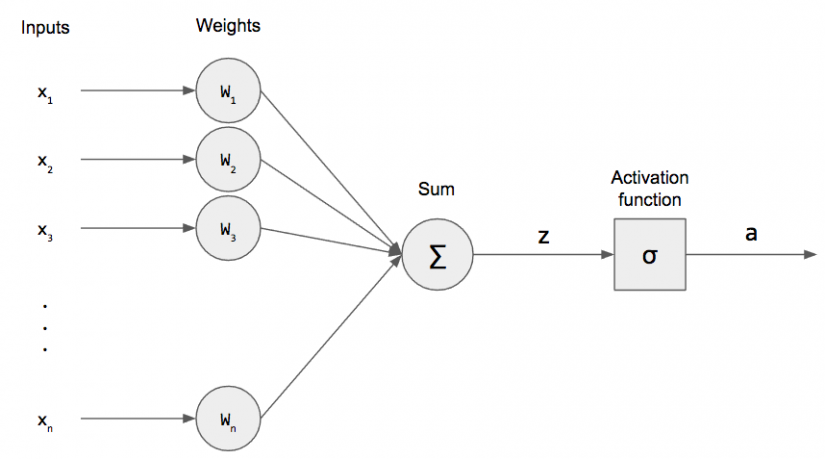
\includegraphics[width=0.6\linewidth,keepaspectratio]{rl69}

{\tiny (Ref: Python Machine Learning - Zenva)}
\end{center}

\end{frame}

%%%%%%%%%%%%%%%%%%%%%%%%%%%%%%%%%%%%%%%%%%%%%%%%%%%%%%%%%%%%%%%%%%%%%%%%%%%%%%%%%
\begin{frame}[fragile]\frametitle{Deep Learning Process}


\begin{itemize}
\item Input is fed into a layer and activated 
\item Result is then fed into next layer, and activated 
\item All the way through to the output
\item Output compared to some target to get cost 
\item  Weights changed to minimize cost (back propagation)
\item Repeat process $\rightarrow$ profit
\end{itemize}

{\tiny (Ref: Modern Reinforcement Learning: Deep Q Learning in PyTorch - Phil Tabor)}

\end{frame}

%%%%%%%%%%%%%%%%%%%%%%%%%%%%%%%%%%%%%%%%%%%%%%%%%%%%%%%%%%%%%%%%%%%%%%%%%%%%%%%%%
\begin{frame}[fragile]\frametitle{Deep Learning for Q Learning}


\begin{itemize}
\item Almost same structure as any standard but with MSE loss, Relu activation and a state-action-reward based Cost function
\item Inputs: states
\item Labels: actions
\item How it was made a supervised like learning problem? when there is no prior labeled data?
\item Target is $r + \gamma max Q(s',a_{max})$
\end{itemize}

{\tiny (Ref: Modern Reinforcement Learning: Deep Q Learning in PyTorch - Phil Tabor)}

\end{frame}

%%%%%%%%%%%%%%%%%%%%%%%%%%%%%%%%%%%%%%%%%%%%%%%%%%%%%%%%%%%%%%%%%%%%%%%%%%%%%%%%%%
\begin{frame}[fragile]\frametitle{Deep RL Algorithms}

There are many different kinds of RL algorithms! This is a non-exhaustive taxonomy (with specific algorithms in blue):
\begin{figure}
\centering
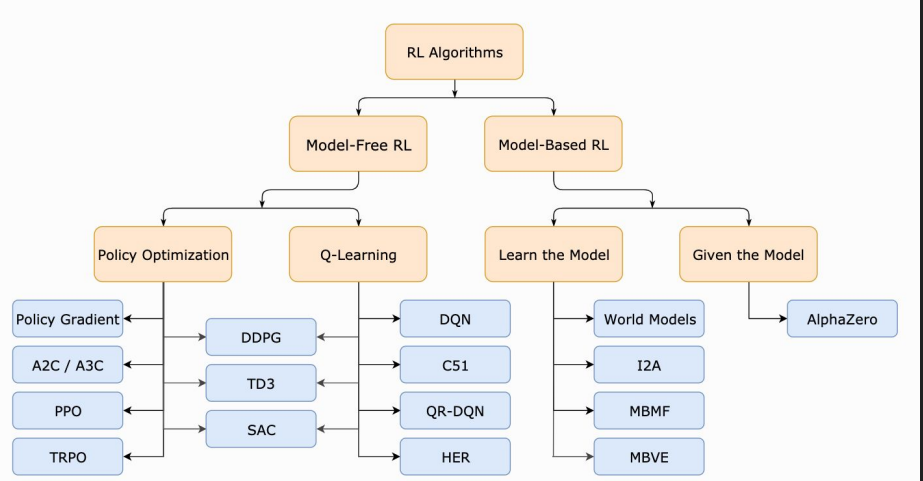
\includegraphics[width=\linewidth]{rl16}
\end{figure}

{\tiny (Ref: Intro to RL - Joshua Achiam)}


\end{frame}

%%%%%%%%%%%%%%%%%%%%%%%%%%%%%%%%%%%%%%%%%%%%%%%%%%%%%%%%%%%%%%%%%%%%%%%%%%%%%%%%%%
\begin{frame}[fragile]\frametitle{Deep RL Algorithms}

Using Model-Free RL Algorithms:
\begin{center}
\begin{tabular}{c|c|c}
Algorithm &  $a$ Discrete &$a$  Continuous \\ \hline
Policy optimization & Yes & Yes \\
DQN / C51 / QR-DQN & Yes & \color{red}{No} \\
DDPG & \color{red}{No} & Yes
\end{tabular}
\end{center}

Using Model-Based RL Algorithms:
\begin{itemize}
\item Learning the model means learning to generate next state and/or reward:
%
\begin{equation*}
\hat{s}_{t+1}, \hat{r}_t = \hat{f}_{\phi}(s_t, a_t)
\end{equation*}
\item Some algorithms may only work with an \textit{exact} model of the environment
\begin{itemize}
\item AlphaZero uses the rules of the game to build its search tree
\end{itemize}
\end{itemize}

{\tiny (Ref: Intro to RL - Joshua Achiam)}


\end{frame}

%%%%%%%%%%%%%%%%%%%%%%%%%%%%%%%%%%%%%%%%%%%%%%%%%%%%%%%%%%%%%%%%%%%%%%%%%%%%%%%%%%
\begin{frame}[fragile]\frametitle{Policy Gradients}

\begin{itemize}
\item An algorithm for training stochastic policies:
\begin{itemize}
\item Run current policy in the environment to collect rollouts
\item Take stochastic gradient ascent on policy performance using the \textbf{policy gradient}:
\begin{align*}
g &= \nabla_{\theta} E_{\tau \sim \pi_{\theta}}{\sum_{t=0}^T r_t} \\
&= E_{\tau \sim \pi_{\theta}}{\sum_{t=0}^T \nabla_{\theta} \log \pi_{\theta}(a_t | s_t) \left(\sum_{t'=t}^T r_{t'}\right)}\\
&\approx \frac{1}{|D|}\sum_{\tau \in D} \sum_{t=0}^T \nabla_{\theta} \log \pi_{\theta}(a_t | s_t) \left(\sum_{t'=t}^T r_{t'}\right)
\end{align*}
\end{itemize}
\item Core idea: push up the probabilities of good actions and push down the probabilities of bad actions
\item Definition: sum of rewards after time $t$ is the \textit{reward-to-go} at time $t$:
%
\begin{equation*}
\hat{R}_t = \sum_{t'=t}^T r_{t'}
\end{equation*}
\end{itemize}

{\tiny (Ref: Intro to RL - Joshua Achiam)}


\end{frame}

%%%%%%%%%%%%%%%%%%%%%%%%%%%%%%%%%%%%%%%%%%%%%%%%%%%%%%%%%%%%%%%%%%%%%%%%%%%%%%%%%%
\begin{frame}[fragile]\frametitle{Example Implementation}

Make the model, loss function, and optimizer:
\begin{lstlisting}
 # make model
 with tf.variable_scope('model'):
     obs_ph = tf.placeholder(shape=(None, obs_dim), dtype=tf.float32)
     net = mlp(obs_ph, hidden_sizes=[hidden_dim]*n_layers)
     logits = tf.layers.dense(net, units=n_acts, activation=None)
     actions = tf.squeeze(tf.multinomial(logits=logits,num_samples=1), axis=1)

 # make loss
 adv_ph = tf.placeholder(shape=(None,), dtype=tf.float32)
 act_ph = tf.placeholder(shape=(None,), dtype=tf.int32)
 action_one_hots = tf.one_hot(act_ph, n_acts)
 log_probs = tf.reduce_sum(action_one_hots * tf.nn.log_softmax(logits), axis=1)
 loss = -tf.reduce_mean(adv_ph * log_probs)

 # make train op
 train_op = tf.train.AdamOptimizer(learning_rate=lr).minimize(loss)

 sess = tf.InteractiveSession()
 sess.run(tf.global_variables_initializer())
\end{lstlisting}


\end{frame}

%%%%%%%%%%%%%%%%%%%%%%%%%%%%%%%%%%%%%%%%%%%%%%%%%%%%%%%%%%%%%%%%%%%%%%%%%%%%%%%%%%
\begin{frame}[fragile]\frametitle{Example Implementation}

One iteration of training:

\begin{lstlisting}
# train model for one iteration
batch_obs, batch_acts, batch_rtgs, batch_rets, batch_lens = [], [], [], [], []
obs, rew, done, ep_rews = env.reset(), 0, False, []
while True:
    batch_obs.append(obs.copy())
    act = sess.run(actions, {obs_ph: obs.reshape(1,-1)})[0]
    obs, rew, done, _ = env.step(act)
    batch_acts.append(act)
    ep_rews.append(rew)
    if done:
        batch_rets.append(sum(ep_rews))
        batch_lens.append(len(ep_rews))
        batch_rtgs += list(discount_cumsum(ep_rews, gamma))
        obs, rew, done, ep_rews = env.reset(), 0, False, []
        if len(batch_obs) > batch_size:
            break
# normalize advs trick:
batch_advs = np.array(batch_rtgs)
batch_advs = (batch_advs - np.mean(batch_advs))/(np.std(batch_advs) + 1e-8)
batch_loss, _ = sess.run([loss,train_op], feed_dict={obs_ph: np.array(batch_obs),
                                                     act_ph: np.array(batch_acts),
                                                     adv_ph: batch_advs})
\end{lstlisting}


\end{frame}

%%%%%%%%%%%%%%%%%%%%%%%%%%%%%%%%%%%%%%%%%%%%%%%%%%%%%%%%%%%%%%%%%%%%%%%%%%%%%%%%%%
\begin{frame}[fragile]\frametitle{Getting Q-Learning to Work (DQN)}

Experience replay:
\begin{itemize}
\item Data distribution changes over time: as your $Q$ function gets better and you \textit{exploit} this, you visit different $(s,a,s',r)$ transitions than you did earlier
\item Stabilize learning by keeping old transitions in a replay buffer, and taking minibatch gradient descent on mix of old and new transitions
\end{itemize}
Target networks:
\begin{itemize}
\item Minimizing Bellman error directly is unstable! 
\item It's \textit{like} regression, but it's not:
%
\begin{equation*}
\min_{\theta} \sum_{(s,a,s',r)\in D} \left(Q_{\theta}(s,a) - y(s',r) \right)^2,
\end{equation*}
%
where the target $y(s',r)$ is
%
\begin{equation*}
y(s',r) = r + \gamma \max_{a'} Q_{\theta}(s',a').
\end{equation*}
%
Targets depend on parameters $\theta$---so an update to $Q$ changes the target!
\item Stabilize it by \textit{holding the target fixed} for a while: keep a separate target network, $Q_{\theta_{targ}}$, and every $k$ steps update $\theta_{targ} \leftarrow \theta$
\end{itemize}
{\tiny (Ref: Intro to RL - Joshua Achiam)}


\end{frame}

%%%%%%%%%%%%%%%%%%%%%%%%%%%%%%%%%%%%%%%%%%%%%%%%%%%%%%%%%%%%%%%%%%%%%%%%%%%%%%%%%%
\begin{frame}[fragile]\frametitle{DQN Pseudocode}

\begin{algorithm}[H]
\tiny
   \caption{Deep Q-Learning}
   \label{alg1}
\begin{algorithmic}
     \STATE Randomly generate $Q$-function parameters $\theta$
     \STATE Set target $Q$-network parameters $\theta_{targ} \leftarrow \theta$
     \STATE Make empty replay buffer $D$
	 \STATE Receive observation $s_0$ from environment
	 \FOR{$t = 0,1,2,...$} 
	 \STATE With probability $\epsilon$, select random action $a_t$; otherwise select $a_t = \arg \max_{a} Q_{\theta}(s_t, a)$
	 \STATE Step environment to get $s_{t+1}, r_t$ and end-of-episode signal $d_t$
	 \STATE Linearly decay $\epsilon$ until it reaches final value $\epsilon_f$
	 \STATE Store $(s_t, a_t, r_t, s_{t+1}, d_t) \to D$
	 \STATE Sample mini-batch of transitions $B = \{(s,a,r,s',d)_i\}$ from $ D$
	 \STATE For each transition in $B$, compute 
	 \begin{equation*}
	 y = \left\{ \begin{array}{ll}
	 r & \text{transition is terminal }(d=\text{True}) \\
	 r + \gamma \max_{a'} Q_{\theta_{targ}}(s', a') & \text{otherwise}
	 \end{array}\right.
	 \end{equation*}
	 \STATE Update $Q$ by gradient descent on regression loss:
	 \begin{equation*}
	 \theta \leftarrow \theta - \alpha \nabla_{\theta} \sum_{(s,a,y)\in B} \left(Q_{\theta}(s,a) - y \right)^2
	 \end{equation*}
	 \IF{ $t \% t_{update} =0$}
	 	\STATE Set $\theta_{targ} \leftarrow \theta$
	 \ENDIF
	\ENDFOR
\end{algorithmic}
\end{algorithm}

{\tiny (Ref: Intro to RL - Joshua Achiam)}


\end{frame}
